\documentclass{ximera}

\input{../../../preamble.tex}


\definecolor{fvdnavy}{HTML}{071D43}
\definecolor{fvdcyan}{HTML}{20BFC6}
\definecolor{fvdcyanlight}{HTML}{EFFCFB}
\definecolor{fvdmagenta}{HTML}{F10D69}
\definecolor{fvdmagentalight}{HTML}{FFF1F7}
\definecolor{fvdtext}{HTML}{163044}





%=================================================
% Pedagogische omgevingen
% PDF: tcolorbox
% HTML: learning-box
%=================================================

\newenvironment{voorkennis}
{%
    \ifdefined\HCode
        \HCode{%
<section class="learning-box learning-box--prior">
<div class="learning-box__header">
<span class="learning-box__icon" aria-hidden="true"></span>
<span class="learning-box__title">Voorkennis</span>
</div>
<div class="learning-box__content">
        }%
        \begin{itemize}
    \else
       \begin{tcolorbox}[
    enhanced,
    breakable,
    colback=fvdcyanlight,
    colframe=fvdcyan,
    coltext=fvdtext,
    boxrule=0.5pt,
    leftrule=4pt,
    arc=4mm,
    outer arc=4mm,
    left=7mm,
    right=6mm,
    top=5mm,
    bottom=5mm,
    before skip=6mm,
    after skip=6mm,
    title=Voorkennis,
    coltitle=fvdcyan,
    fonttitle=\bfseries\Large,
    attach title to upper={\par\smallskip},
    boxed title style={
        empty,
        left=0mm,
        right=0mm,
        top=0mm,
        bottom=0mm
    },
    overlay={
        \draw[
            fvdcyan,
            line width=0.5pt
        ]
        ([xshift=42mm,yshift=-13mm]frame.north west)
        --
        ([xshift=-7mm,yshift=-13mm]frame.north east);
    }
]
        \begin{itemize}
    \fi
}
{%
    \end{itemize}
    \ifdefined\HCode
        \HCode{%
</div>
</section>
        }%
    \else
        \end{tcolorbox}
    \fi
}


\newenvironment{leerdoelen}
{%
    \ifdefined\HCode
        \HCode{%
<section class="learning-box learning-box--goals">
<div class="learning-box__header">
<span class="learning-box__icon" aria-hidden="true"></span>
<span class="learning-box__title">Leerdoelen</span>
</div>
<div class="learning-box__content">
        }%
        \begin{itemize}
    \else
\begin{tcolorbox}[
    enhanced,
    breakable,
    colback=fvdmagentalight,
    colframe=fvdmagenta,
    coltext=fvdtext,
    boxrule=0.5pt,
    leftrule=4pt,
    arc=4mm,
    outer arc=4mm,
    left=7mm,
    right=6mm,
    top=5mm,
    bottom=5mm,
    before skip=6mm,
    after skip=6mm,
    title=Leerdoelen,
    coltitle=fvdmagenta,
    fonttitle=\bfseries\Large,
    attach title to upper={\par\smallskip},
    boxed title style={
        empty,
        left=0mm,
        right=0mm,
        top=0mm,
        bottom=0mm
    },
    overlay={
        \draw[
            fvdmagenta,
            line width=0.5pt
        ]
        ([xshift=42mm,yshift=-13mm]frame.north west)
        --
        ([xshift=-7mm,yshift=-13mm]frame.north east);
    }
]
        \begin{itemize}
    \fi
}
{%
    \end{itemize}
    \ifdefined\HCode
        \HCode{%
</div>
</section>
        }%
    \else
        \end{tcolorbox}
    \fi
}


\addPrintStyle{../../..}

\title{Van werkelijkheid naar wiskunde --- en terug}
\author{Ingmar Herreman}

\begin{abstract}
Wetenschap begint met vragen over de werkelijkheid.
Maar waarnemingen en meetgegevens alleen volstaan meestal niet:
we willen patronen herkennen, verbanden beschrijven, voorspellingen
maken en conclusies kunnen verantwoorden.

In dit hoofdstuk onderzoeken we hoe wiskunde daarbij helpt.
We vertrekken van een concrete wetenschappelijke situatie en bouwen
geleidelijk de weg op van werkelijkheid naar gegevens, van gegevens
naar een wiskundige voorstelling en van daaruit naar een model.

Daarbij staat één idee centraal:

\[
\boxed{
\text{werkelijkheid}
\longrightarrow
\text{wiskunde}
\longrightarrow
\text{betekenis in de werkelijkheid}
}
\]

We leren ook waarom een model nooit de volledige werkelijkheid is,
waarom voorspellingen grenzen hebben en waarom correcte notatie,
eenheden en duidelijke afspraken noodzakelijk zijn.

Deze manier van denken vormt een rode draad doorheen de verdere cursus:
waarnemen, verbanden zoeken, mathematiseren, analyseren, controleren,
interpreteren en kritisch terugkeren naar de oorspronkelijke situatie.
\end{abstract}

\begin{document}

% FVD_CHAPTER_DATA_START
% Automatisch gegenereerd uit index.tex.
% Niet handmatig aanpassen.
\fvdchapterdata{2}{Van werkelijkheid naar wiskunde — en terug}{3}
% FVD_CHAPTER_DATA_END





\maketitle


% ============================================================
% VOORKENNIS EN LEERDOELEN
% ============================================================

\begin{voorkennis}
  \item Je kan informatie aflezen uit een eenvoudige tabel en grafiek.
  \item Je kent courante grootheden en eenheden uit de wetenschapsvakken.
  \item Je kan eenvoudige berekeningen uitvoeren met formules.
  \item Je kan een resultaat in woorden formuleren.
  \item Je kan onderscheid maken tussen een exacte waarde en een afgeronde waarde.
\end{voorkennis}

\begin{leerdoelen}
  \item Je kan in een wetenschappelijke situatie relevante grootheden, waarden en eenheden herkennen.
  \item Je kan uitleggen waarom gegevens slechts een geselecteerde beschrijving van de werkelijkheid vormen.
  \item Je kan een patroon of verband in een tabel of grafiek beschrijven.
  \item Je kan uitleggen wat een wiskundig model is en waarom een model altijd een vereenvoudiging is.
  \item Je kan de begrippen mathematiseren en demathematiseren in een concrete situatie herkennen.
  \item Je kan een wiskundig resultaat terug interpreteren in de oorspronkelijke context.
  \item Je kan onderscheid maken tussen interpoleren en extrapoleren en de betrouwbaarheid ervan kritisch beoordelen.
  \item Je kan eenvoudige grafische voorstellingen kritisch beoordelen.
  \item Je kan uitleggen waarom samenhang niet automatisch causaliteit betekent.
  \item Je kan correct omgaan met grootheden, eenheden en de symbolen $=$ en $\approx$.
  \item Je kan een eenvoudige wetenschappelijke situatie doorlopen volgens een wiskundige modelleercyclus.
\end{leerdoelen}


%%%%%%%%%%%%%%%%%%%%%%%%%%%%%%%%%%%%%%%%%%%%%%%%%%%%%%%%%%%%%%%%%%%%%%
%% 1 WAAROM?
%%%%%%%%%%%%%%%%%%%%%%%%%%%%%%%%%%%%%%%%%%%%%%%%%%%%%%%%%%%%%%%%%%%%%%

\FVDsection{Waarom leer je dit?}

Wiskunde in een wetenschappelijke richting gaat niet alleen over sneller
rekenen of meer formules kennen. We willen wiskunde gebruiken om iets over de werkelijkheid te weten
te komen.

Stel bijvoorbeeld dat je onderzoekt hoe een beker warm water afkoelt.
Om de twee minuten meet je de temperatuur.

\[
\begin{array}{c|ccccccc}
t\;(\mathrm{min})
&0&2&4&6&8&10&12\\ \hline
T\;({}^{\circ}\mathrm C)
&82{,}1&68{,}4&57{,}9&49{,}6&43{,}3&38{,}5&34{,}8
\end{array}
\]

Op het eerste gezicht is dit gewoon een tabel met getallen. Maar een wetenschapper stelt andere vragen:

\begin{itemize}
  \item Hoe verandert de temperatuur?
  \item Is er een herkenbaar patroon?
  \item Kunnen we de temperatuur na $7$ minuten schatten?
  \item Kunnen we voorspellen wat er na $20$ minuten gebeurt?
  \item Welk wiskundig model past bij deze gegevens?
  \item Hoe betrouwbaar zou zo'n voorspelling zijn?
\end{itemize}

De tabel is dus geen eindpunt. Ze is het begin van een onderzoek.

\begin{opmerking}
In deze cursus zullen we vaak dezelfde beweging maken:

\[
\important{
\text{waarnemen}
\longrightarrow
\text{gegevens}
\longrightarrow
\text{wiskundig model}
\longrightarrow
\text{analyse}
\longrightarrow
\text{interpretatie}
}
\]

Die beweging is belangrijk in wiskunde, fysica, chemie, biologie,
engineering en datawetenschap.
\end{opmerking}


%%%%%%%%%%%%%%%%%%%%%%%%%%%%%%%%%%%%%%%%%%%%%%%%%%%%%%%%%%%%%%%%%%%%%%
%% OPENINGSACTIVITEIT
%%%%%%%%%%%%%%%%%%%%%%%%%%%%%%%%%%%%%%%%%%%%%%%%%%%%%%%%%%%%%%%%%%%%%%

\FVDsubsection{Wat kun je al uit gegevens halen?}

\begin{oefening}[Een eerste blik op meetgegevens]{\oefB \ESS}

Gebruik de tabel van het afkoelingsexperiment.

\begin{question}
Welke twee grootheden worden gemeten?

\begin{multipleChoice}
  \choice{massa en temperatuur}
  \choice[correct]{tijd en temperatuur}
  \choice{tijd en volume}
  \choice{temperatuur en energie}
\end{multipleChoice}
\end{question}

\begin{question}
Welke grootheid verandert doordat de tijd verstrijkt?

\begin{multipleChoice}
  \choice{De tijd}
  \choice[correct]{De temperatuur}
\end{multipleChoice}
\end{question}

\begin{question}
Kun je uit de tabel \emph{exact aflezen} wat de temperatuur na
$7$ minuten was?

\begin{multipleChoice}
  \choice{Ja}
  \choice[correct]{Nee}
\end{multipleChoice}
\end{question}

\begin{question}
Welke uitspraak wordt het best door de gegevens ondersteund?

\begin{multipleChoice}
  \choice{De temperatuur stijgt met de tijd.}
  \choice{De temperatuur daalt elke twee minuten met exact hetzelfde aantal graden.}
  \choice[correct]{De temperatuur daalt, maar de daling wordt geleidelijk kleiner.}
  \choice{Na $20$ minuten is de temperatuur zeker $0^\circ\mathrm C$.}
\end{multipleChoice}
\end{question}

\end{oefening}


%%%%%%%%%%%%%%%%%%%%%%%%%%%%%%%%%%%%%%%%%%%%%%%%%%%%%%%%%%%%%%%%%%%%%%
%% 2 WERKELIJKHEID -> GEGEVENS
%%%%%%%%%%%%%%%%%%%%%%%%%%%%%%%%%%%%%%%%%%%%%%%%%%%%%%%%%%%%%%%%%%%%%%

\FVDsection{Van werkelijkheid naar gegevens}

De werkelijkheid verschijnt niet vanzelf in de vorm van een tabel. Een onderzoeker maakt keuzes:

\begin{itemize}
  \item welke verschijnselen worden onderzocht;
  \item welke grootheden relevant zijn;
  \item wat gemeten wordt;
  \item hoe vaak gemeten wordt;
  \item met welk meetinstrument;
  \item met welke nauwkeurigheid.
\end{itemize}

Gegevens zijn dus nooit ``de volledige werkelijkheid''. Ze zijn een geselecteerde en meetbare beschrijving van een deel ervan.



% --------------------------------------------------------------------
% VARIABELEN
% --------------------------------------------------------------------

\FVDsection{Variabelen}

Wanneer een grootheid verschillende waarden kan aannemen, gebruiken we
vaak een letter. In het afkoelingsexperiment schrijven we bijvoorbeeld

\[
t=\text{tijd},
\qquad
T=\text{temperatuur}.
\]

We willen onderzoeken hoe $T$ verandert wanneer $t$ verandert. Daarom beschouwen we hier:

\[
\boxed{
t=\text{onafhankelijke variabele}
}
\]

en

\[
\boxed{
T=\text{afhankelijke variabele}.
}
\]

Later zullen we dergelijke verbanden formeler beschrijven met
\textbf{functies}.




\FVDsection{Een meetwaarde heeft een beperkte nauwkeurigheid}

Wanneer een thermometer aangeeft
\(
57{,}9\,^\circ\mathrm C,
\)
wil dat niet zeggen dat de werkelijke temperatuur mathematisch exact
\(
57{,}900000000\ldots\,^\circ\mathrm C
\) bedraagt.

Een meetinstrument heeft een beperkte nauwkeurigheid. Dat onderscheid is belangrijk:

\[
\boxed{
\text{wiskundige exactheid}
\neq
\text{experimentele nauwkeurigheid}
}
\]

In deze wiskundecursus zullen we niet telkens een volledige
meetonzekerheidsanalyse uitvoeren.

We zullen wel consequent vragen of een getal exact, gemeten,
afgerond of geschat is.


%%%%%%%%%%%%%%%%%%%%%%%%%%%%%%%%%%%%%%%%%%%%%%%%%%%%%%%%%%%%%%%%%%%%%%
%% 4 DATA -> PATROON
%%%%%%%%%%%%%%%%%%%%%%%%%%%%%%%%%%%%%%%%%%%%%%%%%%%%%%%%%%%%%%%%%%%%%%

\FVDsection{Van gegevens naar een patroon}

Een tabel is nuttig om waarden nauwkeurig af te lezen. Een grafiek maakt daarentegen vaak het \emph{gedrag} zichtbaar. Voor het afkoelingsexperiment kunnen we de meetpunten
$(t,T)$ in een assenstelsel plaatsen.

\begin{center}
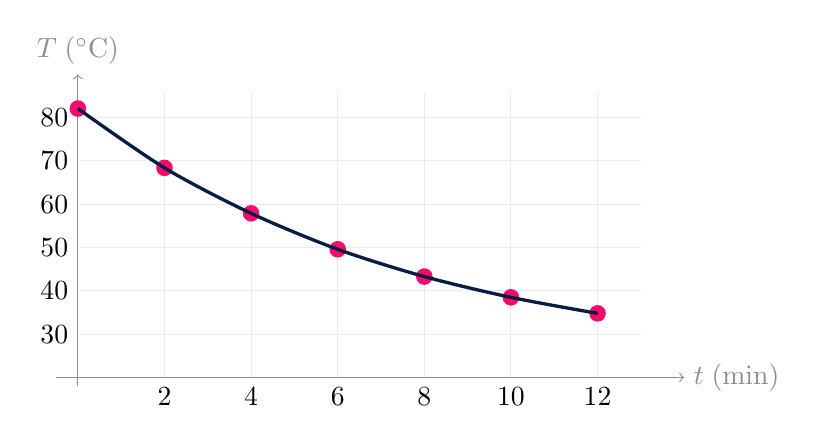
\begin{tikzpicture}[x=0.55cm,y=0.055cm]

  % assen
  \draw[->,black!45] (-0.5,20) -- (14,20)
    node[right] {$t\;(\mathrm{min})$};
  \draw[->,black!45] (0,18) -- (0,90)
    node[above] {$T\;({}^{\circ}\mathrm C)$};

  % hulplijnen
  \foreach \x in {2,4,6,8,10,12}
    \draw[black!8] (\x,20) -- (\x,86);
  \foreach \y in {30,40,50,60,70,80}
    \draw[black!8] (0,\y) -- (13,\y);

  % meetpunten
  \fill[fvdmagenta] (0,82.1) circle (3pt);
  \fill[fvdmagenta] (2,68.4) circle (3pt);
  \fill[fvdmagenta] (4,57.9) circle (3pt);
  \fill[fvdmagenta] (6,49.6) circle (3pt);
  \fill[fvdmagenta] (8,43.3) circle (3pt);
  \fill[fvdmagenta] (10,38.5) circle (3pt);
  \fill[fvdmagenta] (12,34.8) circle (3pt);

  % verbindende curve enkel als visuele gids
  \draw[fvdnavy,very thick,smooth]
    plot coordinates {
      (0,82.1)
      (2,68.4)
      (4,57.9)
      (6,49.6)
      (8,43.3)
      (10,38.5)
      (12,34.8)
    };

  % x labels
  \foreach \x in {2,4,6,8,10,12}
    \node[below] at (\x,20) {\x};

  % y labels
  \foreach \y in {30,40,50,60,70,80}
    \node[left] at (0,\y) {\y};

\end{tikzpicture}
\end{center}

We zien nu onmiddellijk dat:

\begin{itemize}
  \item de temperatuur daalt;
  \item de daling eerst sterk is;
  \item de grafiek later minder snel daalt;
  \item er een duidelijk patroon aanwezig lijkt te zijn.
\end{itemize}

\begin{opmerking}
Een grafiek voegt geen nieuwe meetgegevens toe.

Ze kan wel structuur zichtbaar maken die in een tabel minder
opvallend is.
\end{opmerking}


% --------------------------------------------------------------------
% TABEL OF GRAFIEK
% --------------------------------------------------------------------

\begin{oefening}[Tabel of grafiek?]{\oefB}

Je wilt telkens informatie uit een experiment halen.

\begin{question}
Je wilt de gemeten temperatuur na precies $8$ minuten aflezen.

Welke voorstelling is meestal het handigst?

\begin{multipleChoice}
  \choice[correct]{De tabel}
  \choice{De grafiek}
\end{multipleChoice}
\end{question}

\begin{question}
Je wilt snel zien of de temperatuur stijgt, daalt of ongeveer constant
blijft.

Welke voorstelling is meestal het handigst?

\begin{multipleChoice}
  \choice{De tabel}
  \choice[correct]{De grafiek}
\end{multipleChoice}
\end{question}

\end{oefening}


%%%%%%%%%%%%%%%%%%%%%%%%%%%%%%%%%%%%%%%%%%%%%%%%%%%%%%%%%%%%%%%%%%%%%%
%% 5 MODEL
%%%%%%%%%%%%%%%%%%%%%%%%%%%%%%%%%%%%%%%%%%%%%%%%%%%%%%%%%%%%%%%%%%%%%%

\FVDsection{Van patroon naar wiskundig model}

Wanneer we een patroon herkennen, proberen we het vaak wiskundig te
beschrijven.

\begin{definitie}[Wiskundig model]

Een \textbf{wiskundig model} is een wiskundige beschrijving van
bepaalde aspecten van een werkelijke situatie.

Een model kan bijvoorbeeld bestaan uit:

\begin{itemize}
  \item een tabel;
  \item een grafiek;
  \item een formule;
  \item een verzameling vergelijkingen;
  \item een kansmodel;
  \item een matrixmodel.
\end{itemize}

\end{definitie}

Het woord \emph{bepaalde} is belangrijk. Een model probeert niet de volledige werkelijkheid te kopiëren. Het kiest precies die eigenschappen die voor de onderzoeksvraag belangrijk zijn.


%%%%%%%%%%%%%%%%%%%%%%%%%%%%%%%%%%%%%%%%%%%%%%%%%%%%%%%%%%%%%%%%%%%%%%
%% MATHEMATISEREN
%%%%%%%%%%%%%%%%%%%%%%%%%%%%%%%%%%%%%%%%%%%%%%%%%%%%%%%%%%%%%%%%%%%%%%

\FVDsubsection{Mathematiseren}

De stap van de werkelijke situatie naar een wiskundige beschrijving
noemen we \textbf{mathematiseren}.

\[
\important{
\text{werkelijkheid}
\longrightarrow
\text{wiskundig model}
}
\]

Daarbij kunnen we bijvoorbeeld:

\begin{itemize}
  \item relevante grootheden kiezen;
  \item variabelen invoeren;
  \item gegevens in een tabel plaatsen;
  \item een grafiek tekenen;
  \item een formule zoeken;
  \item aannames formuleren.
\end{itemize}


\begin{voorbeeld}

Een auto rijdt op een rechte weg.

We willen niet de kleur, het merk, de temperatuur van de motor en de
muziek in de auto beschrijven.

We onderzoeken alleen de beweging.

Dan kunnen we bijvoorbeeld kiezen voor:

\[
t=\text{tijd},
\qquad
s=\text{positie}.
\]

De werkelijke beweging wordt zo vertaald naar een wiskundig verband
tussen $t$ en $s$.

Dat is mathematiseren.

\end{voorbeeld}


%%%%%%%%%%%%%%%%%%%%%%%%%%%%%%%%%%%%%%%%%%%%%%%%%%%%%%%%%%%%%%%%%%%%%%
%% DEMATHEMATISEREN
%%%%%%%%%%%%%%%%%%%%%%%%%%%%%%%%%%%%%%%%%%%%%%%%%%%%%%%%%%%%%%%%%%%%%%

\FVDsubsection{Demathematiseren}

Na een berekening moeten we terugkeren naar de oorspronkelijke
situatie. Die stap noemen we \textbf{demathematiseren}.

\[
\important{
\text{wiskundig resultaat}
\longrightarrow
\text{betekenis in de werkelijkheid}
}
\]

\begin{voorbeeld}

Stel dat een model voor de afgelegde afstand gegeven wordt door

\[
s(t)=4{,}9t^2,
\]

waarbij $t$ in seconden en $s$ in meter wordt uitgedrukt.

Voor $t=2$ vinden we:

\[
s(2)=4{,}9\cdot2^2=19{,}6.
\]

Het getal
\(
19{,}6
\)
is nog geen volledig antwoord.

In de situatie betekent het:

\[
\boxed{
\text{na }2\,\mathrm s\text{ is volgens het model }19{,}6\,\mathrm m
\text{ afgelegd.}
}
\]

\end{voorbeeld}


\begin{opmerking}
Bij toepassingen eindigt een oplossing dus niet noodzakelijk bij

\[
x=3{,}2.
\]

We vragen altijd:

\[
\boxed{\text{Wat betekent dit getal in de oorspronkelijke situatie?}}
\]
\end{opmerking}


\begin{oefening}[Van resultaat naar betekenis]{\oefB \ESS}

Een model voor de massa $m(t)$ van een stof geeft

\[
m(6)=24{,}7,
\]

waarbij $t$ in uren en $m$ in gram wordt uitgedrukt.

Welke interpretatie is correct?

\begin{multipleChoice}
  \choice{Na $24{,}7$ uur is de massa $6$ gram.}
  \choice[correct]{Na $6$ uur is de massa volgens het model $24{,}7$ gram.}
  \choice{De massa neemt elke $6$ uur met $24{,}7$ gram toe.}
  \choice{De massa is altijd $24{,}7$ gram.}
\end{multipleChoice}

\end{oefening}


%%%%%%%%%%%%%%%%%%%%%%%%%%%%%%%%%%%%%%%%%%%%%%%%%%%%%%%%%%%%%%%%%%%%%%
%% 6 MODEL IS NIET WERKELIJKHEID
%%%%%%%%%%%%%%%%%%%%%%%%%%%%%%%%%%%%%%%%%%%%%%%%%%%%%%%%%%%%%%%%%%%%%%

\FVDsection{Een model is niet de werkelijkheid}

Een formule kan zeer nauwkeurig zijn zonder de volledige werkelijkheid
te beschrijven. Beschouw bijvoorbeeld het vereenvoudigde model voor vrije val:

\[
h(t)=h_0-\frac12gt^2.
\]

Zo'n model kan gebaseerd zijn op aannames zoals:

\begin{itemize}
  \item de luchtweerstand wordt verwaarloosd;
  \item $g$ wordt constant genomen;
  \item het voorwerp wordt als een punt beschouwd;
  \item andere invloeden worden niet meegenomen.
\end{itemize}

Toch kan het model in veel situaties zeer bruikbaar zijn.

\begin{opmerking}
Een model hoeft niet perfect te zijn om nuttig te zijn.

De juiste vraag is:

\[
\important{
\text{Is dit model geschikt voor de vraag die we willen beantwoorden?}
}
\]
\end{opmerking}



%%%%%%%%%%%%%%%%%%%%%%%%%%%%%%%%%%%%%%%%%%%%%%%%%%%%%%%%%%%%%%%%%%%%%%
%% 7 VIER FUNCTIES VAN WISKUNDE
%%%%%%%%%%%%%%%%%%%%%%%%%%%%%%%%%%%%%%%%%%%%%%%%%%%%%%%%%%%%%%%%%%%%%%

\FVDsection{Wat doet wiskunde in de wetenschappen?}

Wiskunde vervult verschillende rollen. Vier ervan zullen in deze cursus voortdurend terugkomen:

\[
\boxed{
\text{beschrijven}
\qquad
\text{verbanden onderzoeken}
\qquad
\text{voorspellen}
\qquad
\text{optimaliseren}
}
\]


% --------------------------------------------------------------------
% BESCHRIJVEN
% --------------------------------------------------------------------

\FVDsubsection{Beschrijven}
\begin{itemize}
  \item Een bewegend voorwerp kunnen we beschrijven door zijn positie $s$ als
  functie van de tijd $t$.
  \item Een chemisch proces kan beschreven worden door een concentratie als
  functie van de tijd.
  \item Een biologisch systeem kan beschreven worden door het aantal organismen
  doorheen de tijd.
\end{itemize}

Wiskunde geeft ons een taal om veranderingen systematisch te
beschrijven.


% --------------------------------------------------------------------
% VERBAND
% --------------------------------------------------------------------

\FVDsubsection{Verbanden onderzoeken}

In wetenschappelijke experimenten onderzoeken we vaak hoe twee
grootheden samenhangen.

Bijvoorbeeld:

\[
U \longleftrightarrow I
\]

voor spanning en stroomsterkte,

of

\[
m \longleftrightarrow V
\]

voor massa en volume.

Later in deze module zullen we dergelijke verbanden onderzoeken met
spreidingsdiagrammen, correlatie en regressie.


% --------------------------------------------------------------------
% VOORSPELLEN
% --------------------------------------------------------------------

\FVDsubsection{Voorspellen}

Een model kan ons helpen een waarde te schatten die we niet rechtstreeks
gemeten hebben.

Bijvoorbeeld:

\begin{itemize}
  \item de temperatuur na een bepaald tijdstip;
  \item de positie van een bewegend voorwerp;
  \item de hoeveelheid radioactieve stof na enkele jaren;
  \item de verwachte opbrengst van een systeem.
\end{itemize}

Een voorspelling is echter nooit automatisch betrouwbaar. Daarvoor moeten we ook weten \emph{waar} en \emph{onder welke
voorwaarden} het model gebruikt wordt.


% --------------------------------------------------------------------
% OPTIMALISEREN
% --------------------------------------------------------------------

\FVDsubsection{Optimaliseren}

Wiskunde helpt ook om een beste keuze te zoeken.

Bijvoorbeeld:

\begin{itemize}
  \item Welke verpakking gebruikt het minste materiaal?
  \item Welke route vraagt de minste tijd?
  \item Bij welke instelling is het rendement maximaal?
  \item Welke afmetingen geven een zo groot mogelijk volume?
\end{itemize}

Later zullen afgeleiden een krachtig hulpmiddel worden om zulke
extremumproblemen systematisch op te lossen.


%%%%%%%%%%%%%%%%%%%%%%%%%%%%%%%%%%%%%%%%%%%%%%%%%%%%%%%%%%%%%%%%%%%%%%
%% 8 INTERPOLATIE / EXTRAPOLATIE
%%%%%%%%%%%%%%%%%%%%%%%%%%%%%%%%%%%%%%%%%%%%%%%%%%%%%%%%%%%%%%%%%%%%%%

\FVDsection{Voorspellen binnen en buiten de gegevens}

Niet elke voorspelling is even gewaagd.

\begin{definitie}[Interpoleren]

\textbf{Interpoleren} betekent een waarde schatten
\emph{tussen} bekende of gemeten waarden.

\end{definitie}

In ons afkoelingsexperiment is een schatting van de temperatuur na
$7$ minuten een interpolatie, want

\[
6<7<8.
\]

\begin{definitie}[Extrapoleren]

\textbf{Extrapoleren} betekent een waarde voorspellen
\emph{buiten} het gebied waarin gegevens beschikbaar zijn.

\end{definitie}

Een voorspelling voor $t=30$ minuten op basis van metingen tot
$t=12$ minuten is extrapolatie.

\begin{opmerking}
Extrapolatie is vaak riskanter dan interpolatie.

Een patroon dat binnen het gemeten gebied goed werkt, hoeft buiten dat
gebied niet te blijven gelden.
\end{opmerking}


\begin{oefening}[Interpoleren of extrapoleren?]{\oefB \ESS}

Een experiment bevat metingen voor

\[
0\leq t\leq 20.
\]

\begin{question}
Een waarde wordt geschat voor $t=13$.

\begin{multipleChoice}
  \choice[correct]{interpolatie}
  \choice{extrapolatie}
\end{multipleChoice}
\end{question}

\begin{question}
Een waarde wordt voorspeld voor $t=50$.

\begin{multipleChoice}
  \choice{interpolatie}
  \choice[correct]{extrapolatie}
\end{multipleChoice}
\end{question}

\end{oefening}


\begin{oefening}[Een model te ver doortrekken]{\oefU \ESS}

Een groeimodel werd opgesteld met gegevens uit de eerste
$20$ levensdagen van een jonge plant.

Een leerling gebruikt hetzelfde model om de hoogte van de plant
na $10$ jaar te voorspellen.

\begin{question}
Waarom is die voorspelling problematisch?

\begin{multipleChoice}
  \choice{Een wiskundig model mag nooit gebruikt worden om te voorspellen.}
  \choice{Een plant kan niet gemeten worden.}
  \choice[correct]{De leerling extrapoleert zeer ver buiten het gebied waarop het model gebaseerd is.}
  \choice{Een model mag alleen gehele getallen bevatten.}
\end{multipleChoice}
\end{question}

\begin{question}
Welke bijkomende vraag is wetenschappelijk belangrijk?

\begin{multipleChoice}
  \choice{Is de formule mooi geschreven?}
  \choice[correct]{Zijn de aannames van het model over zo'n lange periode nog redelijk?}
  \choice{Heeft de leerling een blauwe pen gebruikt?}
\end{multipleChoice}
\end{question}

\end{oefening}


%%%%%%%%%%%%%%%%%%%%%%%%%%%%%%%%%%%%%%%%%%%%%%%%%%%%%%%%%%%%%%%%%%%%%%
%% 9 KRITISCH LEZEN VAN GRAFIEKEN
%%%%%%%%%%%%%%%%%%%%%%%%%%%%%%%%%%%%%%%%%%%%%%%%%%%%%%%%%%%%%%%%%%%%%%


\FVDsection{Een grafiek kan correct zijn en toch misleiden}

Grafieken maken patronen zichtbaar. Maar de manier waarop een grafiek wordt
voorgesteld, beïnvloedt ook de indruk die we krijgen.

Stel dat twee waarden respectievelijk
\[
98
\qquad\text{en}\qquad
102
\]
zijn.

Bekijk hoe dezelfde gegevens er op twee verschillende verticale schalen
uitzien.

\begin{center}
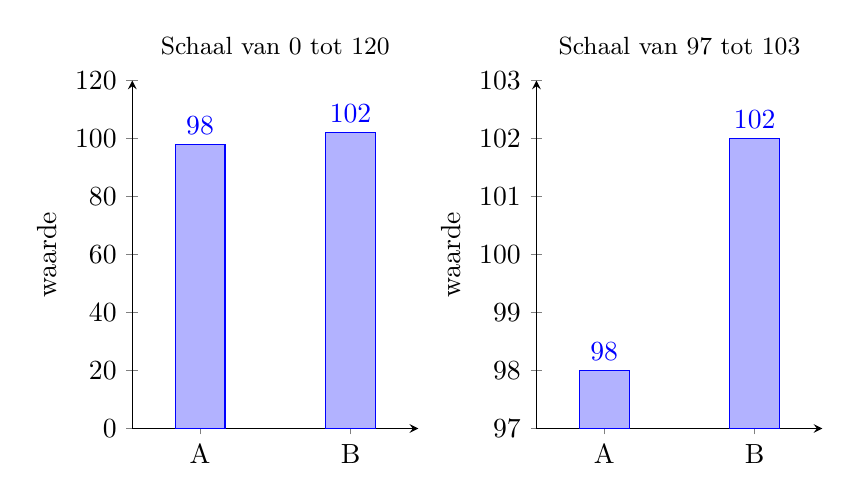
\begin{tikzpicture}

% ---------------------------------------------------------
% Grafiek 1: verticale schaal van 0 tot 120
% ---------------------------------------------------------
\begin{axis}[
    name=plotA,
    width=0.43\textwidth,
    height=6cm,
    ybar,
    bar width=18pt,
    ymin=0,
    ymax=120,
    ytick={0,20,40,60,80,100,120},
    xtick={1,2},
    xticklabels={A,B},
    ylabel={waarde},
    title={\small Schaal van 0 tot 120},
    axis lines=left,
    enlarge x limits=0.45,
    nodes near coords,
    nodes near coords align={vertical},
    clip=false
]
\addplot coordinates {
    (1,98)
    (2,102)
};
\end{axis}

% ---------------------------------------------------------
% Grafiek 2: verticale schaal van 97 tot 103
% ---------------------------------------------------------
\begin{axis}[
    at={(plotA.east)},
    anchor=west,
    xshift=1.5cm,
    width=0.43\textwidth,
    height=6cm,
    ybar,
    bar width=18pt,
    ymin=97,
    ymax=103,
    ytick={97,98,99,100,101,102,103},
    xtick={1,2},
    xticklabels={A,B},
    ylabel={waarde},
    title={\small Schaal van 97 tot 103},
    axis lines=left,
    enlarge x limits=0.45,
    nodes near coords,
    nodes near coords align={vertical},
    clip=false
]
\addplot coordinates {
    (1,98)
    (2,102)
};
\end{axis}

\end{tikzpicture}
\end{center}

In de linkergrafiek lijkt het verschil tussen beide waarden klein.
In de rechtergrafiek lijkt datzelfde verschil plots zeer groot.

Toch stellen beide grafieken exact dezelfde gegevens voor.

\begin{center}
    \textbf{De gegevens zijn niet veranderd. De voorstelling wel.}
\end{center}

Een grafiek kan dus wiskundig correct zijn en toch een misleidende indruk
wekken. Let daarom niet alleen op de vorm van een grafiek, maar controleer
ook altijd de \textbf{schaal} en het \textbf{bereik van de assen}.


\begin{opmerking}
Lees een grafiek daarom nooit alleen ``op het zicht''.

Controleer minstens:

\begin{itemize}
  \item welke grootheden op de assen staan;
  \item welke eenheden gebruikt worden;
  \item welke schaal gekozen is;
  \item waar de assen beginnen;
  \item welke gegevens wel en niet zichtbaar zijn.
\end{itemize}
\end{opmerking}


\begin{oefening}[De schaal beïnvloedt de indruk]{\oefU \ESS}

Twee grafieken stellen exact dezelfde gegevens voor.

De eerste verticale as loopt van $0$ tot $100$.

De tweede verticale as loopt van $80$ tot $100$.

\begin{question}
Waarom kunnen beide grafieken een verschillende indruk geven?

\begin{multipleChoice}
  \choice{De meetwaarden worden automatisch anders.}
  \choice[correct]{De tweede schaal vergroot kleine verticale verschillen visueel uit.}
  \choice{Een grafiek die niet bij nul begint is altijd fout.}
  \choice{De eerste grafiek bevat minder gegevens.}
\end{multipleChoice}
\end{question}

\begin{question}
Welke conclusie is het meest verantwoord?

\begin{multipleChoice}
  \choice{Een grafiek moet altijd bij nul beginnen.}
  \choice{De schaal van een grafiek is onbelangrijk.}
  \choice[correct]{De schaal moet mee beoordeeld worden wanneer we een grafiek interpreteren.}
\end{multipleChoice}
\end{question}

\end{oefening}


%%%%%%%%%%%%%%%%%%%%%%%%%%%%%%%%%%%%%%%%%%%%%%%%%%%%%%%%%%%%%%%%%%%%%%
%% 10 SAMENHANG EN CAUSALITEIT
%%%%%%%%%%%%%%%%%%%%%%%%%%%%%%%%%%%%%%%%%%%%%%%%%%%%%%%%%%%%%%%%%%%%%%

\FVDsection{Samenhang is nog geen oorzaak}

Wanneer twee grootheden samen veranderen, spreken we van een
\textbf{samenhang}. Maar daaruit volgt niet automatisch dat de ene grootheid de andere
\emph{veroorzaakt}. Stel bijvoorbeeld dat in warme zomermaanden zowel de verkoop van ijsjes
als het aantal mensen aan openluchtzwembaden stijgt.

Daaruit volgt niet dat meer ijsjes kopen rechtstreeks veroorzaakt dat
meer mensen gaan zwemmen.

Een derde factor --- \textbf{de temperatuur} --- beïnvloedt beide.

\begin{opmerking}
Een gevonden verband kan een belangrijke aanwijzing zijn.

Maar:

\[
\important{
\text{samenhang}
\not\Longrightarrow
\text{oorzaak-gevolg}
}
\]

Om causaliteit te besluiten is bijkomend wetenschappelijk onderzoek
nodig.
\end{opmerking}


\begin{oefening}[Samenhang of oorzaak?]{\oefU}

Een onderzoek toont dat leerlingen die gemiddeld langer slapen,
gemiddeld betere resultaten behalen.

Een leerling besluit:

\begin{center}
``Meer slapen veroorzaakt dus noodzakelijk betere punten.''
\end{center}

\begin{question}
Is die conclusie verantwoord op basis van alleen deze samenhang?

\begin{multipleChoice}
  \choice{Ja}
  \choice[correct]{Nee}
\end{multipleChoice}
\end{question}

\begin{question}
Welke reden is het best?

\begin{multipleChoice}
  \choice{Twee grootheden kunnen nooit samenhangen.}
  \choice[correct]{Andere factoren kunnen beide grootheden beïnvloeden en samenhang alleen bewijst geen causaliteit.}
  \choice{Slaap kan niet gemeten worden.}
\end{multipleChoice}
\end{question}

\end{oefening}







\FVDsection{Van werkelijkheid naar wiskunde --- en terug}


\begin{oefening}[Een bewegend object onderzoeken]{\oefU \ESS}

Tijdens een experiment wordt om de $10$ seconden de afstand gemeten
die een klein bewegend object vanaf zijn startpunt heeft afgelegd.

\[
\begin{array}{c|cccccc}
t\;(\mathrm s)
&0&10&20&30&40&50\\ \hline
s\;(\mathrm m)
&0&4{,}8&10{,}1&15{,}0&20{,}2&24{,}9
\end{array}
\]

\begin{question}
Welke twee grootheden worden onderzocht?

\begin{multipleChoice}
  \choice{tijd en snelheid}
  \choice[correct]{tijd en afgelegde afstand}
  \choice{massa en afstand}
  \choice{afstand en temperatuur}
\end{multipleChoice}
\end{question}

\begin{question}
Welke grootheid is hier de onafhankelijke variabele?

\begin{multipleChoice}
  \choice[correct]{de tijd $t$}
  \choice{de afstand $s$}
\end{multipleChoice}
\end{question}

\begin{question}
Welke beschrijving past het best bij de gegevens?

\begin{multipleChoice}
  \choice{De afstand blijft ongeveer constant.}
  \choice{De afstand neemt steeds sneller toe.}
  \choice[correct]{De afstand neemt ongeveer gelijkmatig toe met de tijd.}
  \choice{De afstand daalt.}
\end{multipleChoice}
\end{question}

\begin{question}
Een leerling schat voor $t=25\,\mathrm s$:

\[
s\approx12{,}5\,\mathrm m.
\]

Is dit interpolatie of extrapolatie?

\begin{multipleChoice}
  \choice[correct]{interpolatie}
  \choice{extrapolatie}
\end{multipleChoice}
\end{question}

\begin{question}
Dezelfde leerling gebruikt het patroon om de afstand na
$5000\,\mathrm s$ te voorspellen.

Welke uitspraak is correct?

\begin{multipleChoice}
  \choice{De voorspelling is zeker correct omdat de eerste meetpunten bijna lineair liggen.}
  \choice[correct]{De voorspelling is een zeer verre extrapolatie en is zonder bijkomende informatie niet betrouwbaar.}
  \choice{Extrapoleren levert altijd exact dezelfde waarde als meten.}
\end{multipleChoice}
\end{question}

\begin{question}
Een leerling beweert:

\begin{center}
``Omdat de meetpunten bijna op een rechte lijn liggen,
bewoog het object op elk ogenblik exact met dezelfde snelheid.''
\end{center}

Welke beoordeling is het best?

\begin{multipleChoice}
  \choice[correct]{De conclusie is te sterk: de gegevens ondersteunen een ongeveer lineair model, maar bewijzen geen exact constante snelheid op elk ogenblik.}
  \choice{De conclusie is noodzakelijk juist.}
  \choice{Uit een tabel mag je nooit iets over beweging besluiten.}
\end{multipleChoice}
\end{question}

\begin{question}
Wat zou een wiskundig model in deze situatie moeten beschrijven?

\begin{multipleChoice}
  \choice{De kleur en vorm van het object.}
  \choice[correct]{Hoe de afgelegde afstand $s$ verandert in functie van de tijd $t$.}
  \choice{Alle eigenschappen van het object en zijn omgeving.}
\end{multipleChoice}
\end{question}

\end{oefening}


\end{document}
